%!TEX TS-program = xelatex
%!TEX encoding = UTF-8 Unicode

\documentclass[11pt,tikz,border=1]{standalone}
\usetikzlibrary{positioning}

\begin{document}
  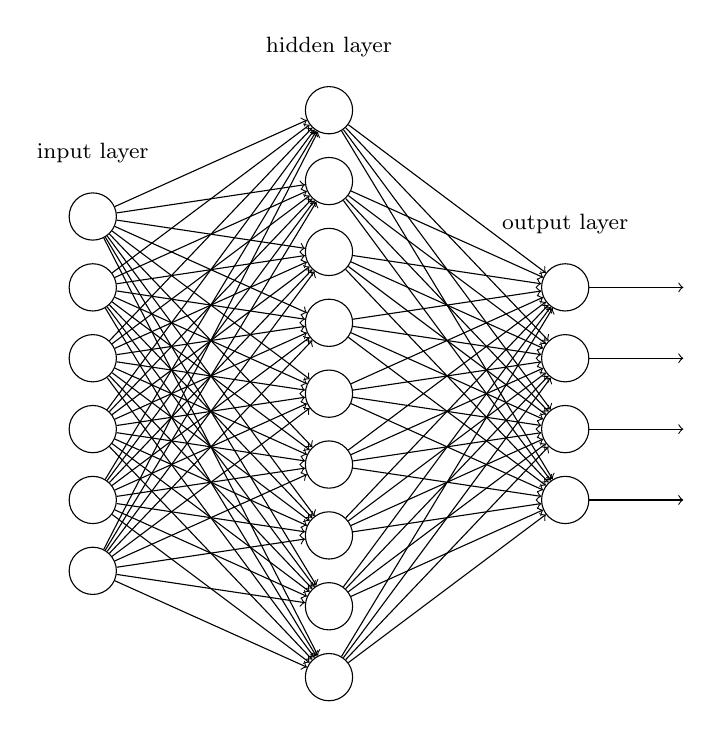
\begin{tikzpicture}[
    neuron/.style={circle,draw,inner sep=0pt,minimum size=6mm},
    font=\footnotesize
    ]

    % input layer:
    \foreach \y in {0,...,5}
      \node(i\y) at (0, \y * 0.9 + 1.35) [neuron] {};

    % hidden layer:
    \foreach \y in {0,...,8}
      \node(h\y) at (3, \y * 0.9) [neuron] {};

        
    % output layer:
    \foreach \y in {0,...,3}
      \node(o\y) at (6, \y * 0.9 + 2.25) [neuron] {};

    % connections
    \foreach \x in {0,...,5}
        \foreach \y in {0,...,8}
            \draw[->] (i\x) to (h\y);

    \foreach \x in {0,...,8}
        \foreach \y in {0,...,3}
            \draw[->] (h\x) to (o\y);
    
    \foreach \y in {0,...,3}
        \draw[->] (o\y) -- ++(1.5,0);

    \node [above=0.25 of i5] {input layer};
    \node [above=0.25 of h8] {hidden layer};
    \node [above=0.25 of o3] {output layer};

  \end{tikzpicture} 
\end{document}
